\section{git}

\begin{frame}
\begin{center}
\includegraphics{git-logo.pdf}\end{center}
\end{frame}

\begin{frame}
\begin{quote}git : con, connard, salaud\end{quote}
\begin{flushright}--- WordReference.com\end{flushright}

\begin{quote}Je ne suis qu'un sale égocentrique, donc j'appelle tous mes projets d'après ma propre personne. D'abord Linux, puis Git.\end{quote}
\begin{flushright}--- Linus Torvalds\end{flushright}
\end{frame}

\begin{frame}{Contexte de création}
Linux utilisait BitKeeper

Utilisation de BitKeeper devenue payante $\Rightarrow$ changement de gestionnaire de version
\end{frame}

\begin{frame}{Sélection d'un remplaçant}
Critères requis :
\begin{itemize}
\item fiabilité / robustesse (pas de corruption de dépôt)
\item haute performance (Linux est un gros projet)
\item distribué
\item gratuité
\end{itemize}

Aucun gestionnaire de version viable…
\end{frame}

\begin{frame}{Cahier des charges}
Design : 
\begin{itemize}
	\item Dépôt : graphe orienté acyclique de commissions
	\item Faire l'opposé complet de CVS, s'inspirer de BitKeeper
	\item Suivre non pas des fichiers individuels mais un contenu (tout le dépôt) d'un coup (des fichiers individuels ne sont pas intéressants, une collection de fichiers l'est)
	\item Les commissions sont identifiés par un hash (SHA-1)
	\item Ce hash permet de garantir qu'il n'y a aucune corruption dans le dépôt
\end{itemize}

Création de git par Linus Torvalds (sortie initiale : 7 avril 2005)
\end{frame}

\begin{frame}{Les états}
Les fichiers peuvent être dans trois états pour un dépôt :
\begin{itemize}
	\item Dans le dossier de travail
	\item Dans la zone de préparation
	\item Dans le dépôt
\end{itemize}
\begin{center}
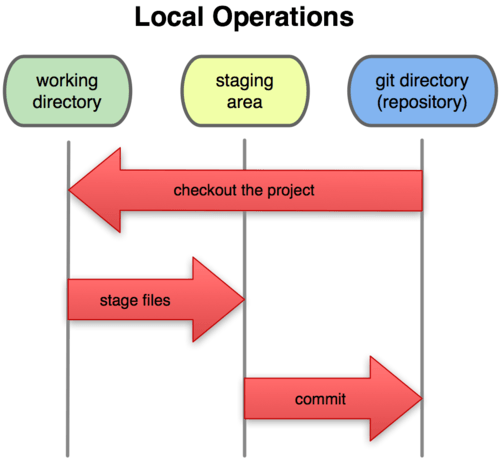
\includegraphics[scale=0.3]{18333fig0106-tn.png}
\end{center}
\end{frame}

\begin{frame}{Cycle de travail classique}{Travail sur une fonctionnalité x}
On crée une branche par fonctionnalité en cours de développement, au nom de la fonctionnalité :
\begin{itemize}
	\item \texttt{git branch x}
\end{itemize}

On se déplace vers cette branche :
\begin{itemize}
	\item \texttt{git checkout x}
\end{itemize}

Lorsqu'on vérifie une branche, le contenu du dossier de travail est remplacé par celui de la branche.

\texttt{master} est la branche par défaut :
\begin{itemize}
	\item \texttt{git checkout master}
\end{itemize}
\end{frame}

\begin{frame}{Cycle de travail classique}{Modification de la branche}
Modifier le dépôt local :

Ajout des nouveaux fichiers et  des fichiers modifiés en zone de préparation :
\begin{itemize}
	\item \texttt{git add fichier1 fichier2}
\end{itemize}

Commission des changements dans le dépôt local (à faire le plus souvent possible) :
\begin{itemize}
	\item \texttt{git commit -m "Message succint décrivant les changements."}
\end{itemize}

Quand la modification est prête :
\begin{itemize}
	\item \texttt{git push}
\end{itemize}

\end{frame}

\begin{frame}{Outils graphiques}
\begin{center}
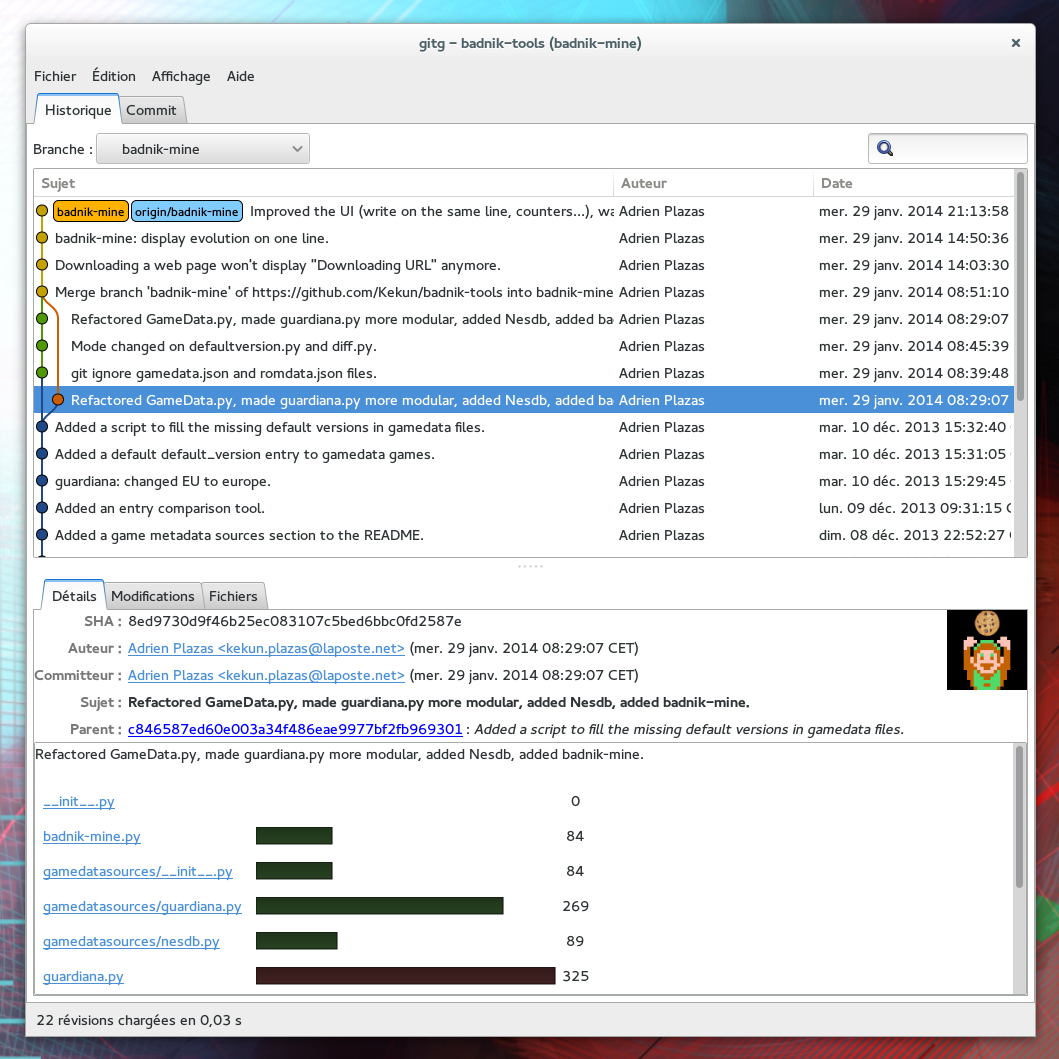
\includegraphics[scale=0.21]{gitg.png}
\end{center}
\end{frame}

\begin{frame}{Essayer git}
http://try.github.io/ permet de tester git en apprenant ses commandes dans un faux terminal.
\end{frame}

%http://try.github.io/

